\chapter{УСТАНОВКА ОПЕРАЦИОННОЙ СИСТЕМЫ СЕМЕЙСТВА LINUX}

\section{Цель работы}

Целью данной лабораторной работы является изучение процесса установки операционной системы семейства Linux, знакомство с интерфейсом и особенностями работы в данной среде.

\section{Выбор дистрибутива}

Для выполнения лабораторной работы был выбран дистрибутив Ubuntu 22.04 LTS. Ubuntu является одним из самых популярных и дружелюбных к пользователю дистрибутивов Linux, основанным на Debian. Выбор обусловлен следующими факторами:

\begin{itemize}
    \item Широкая поддержка сообщества и документации
    \item Стабильность и надежность (LTS версия)
    \item Простота установки и настройки
    \item Большое количество предустановленного программного обеспечения
\end{itemize}

\section{Процесс установки}

\subsection{Подготовка к установке}

Перед установкой Ubuntu были выполнены следующие подготовительные действия:

\begin{enumerate}
    \item Скачан образ Ubuntu 22.04 LTS с официального сайта
    \item Создан загрузочный USB-накопитель с помощью утилиты Rufus
    \item Настроена виртуальная машина в VirtualBox с выделением 4 ГБ оперативной памяти и 25 ГБ дискового пространства
\end{enumerate}

\subsection{Установка системы}

Процесс установки Ubuntu прошел в несколько этапов:

\begin{enumerate}
    \item \textbf{Загрузка с USB-накопителя} --- система успешно загрузилась с созданного загрузочного носителя
    \item \textbf{Выбор языка и раскладки клавиатуры} --- установлен русский язык и соответствующая раскладка
    \item \textbf{Настройка сети} --- подключение к Wi-Fi сети выполнено без проблем
    \item \textbf{Разметка диска} --- выбран автоматический режим разметки с шифрованием диска
    \item \textbf{Создание пользователя} --- создан пользователь с правами администратора
    \item \textbf{Установка дополнительного ПО} --- выбрана установка дополнительных драйверов и мультимедиа кодеков
\end{enumerate}

Общее время установки составило приблизительно 25-30 минут.

\begin{figure}[H]
    \centering
    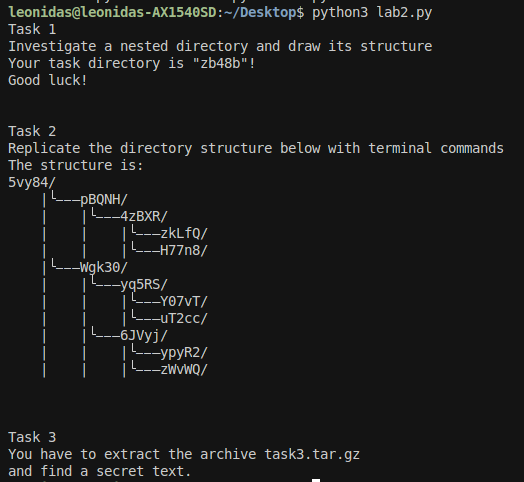
\includegraphics[width=0.8\textwidth]{image.png}
    \caption{Рабочий стол Ubuntu после успешной установки}
    \label{fig:ubuntu_desktop}
\end{figure}

\section{Исследование интерфейса и функциональности}

\subsection{Первые впечатления}

После установки и первого входа в систему были исследованы основные элементы интерфейса Ubuntu:

\begin{itemize}
    \item \textbf{Рабочий стол} --- чистый и минималистичный интерфейс с панелью задач внизу экрана
    \item \textbf{Файловый менеджер} --- интуитивно понятный интерфейс, похожий на проводник Windows
    \item \textbf{Центр приложений} --- удобный магазин приложений с возможностью установки программ
    \item \textbf{Терминал} --- мощный инструмент для работы с командной строкой
\end{itemize}

\subsection{Сравнение с другими ОС}

При сравнении Ubuntu с другими операционными системами были выявлены следующие особенности:

\textbf{Сходства с Windows:}
\begin{itemize}
    \item Графический интерфейс с окнами и панелью задач
    \item Возможность установки программ через графический интерфейс
    \item Поддержка большинства популярных форматов файлов
    \item Наличие файлового менеджера с привычной структурой
\end{itemize}

\textbf{Отличия от Windows:}
\begin{itemize}
    \item Отсутствие реестра --- настройки хранятся в конфигурационных файлах
    \item Централизованное управление пакетами через менеджер пакетов
    \item Более гибкая система прав доступа
    \item Возможность глубокой кастомизации интерфейса
    \item Встроенная поддержка виртуализации и контейнеризации
\end{itemize}

\subsection{Непривычные аспекты}

Наиболее непривычными для пользователя Windows оказались:

\begin{enumerate}
    \item \textbf{Работа с правами доступа} --- необходимость использования команды \texttt{sudo} для выполнения административных задач
    \item \textbf{Установка программ через терминал} --- команды \texttt{apt update} и \texttt{apt install} для управления пакетами
    \item \textbf{Структура файловой системы} --- иерархия каталогов отличается от Windows (например, \texttt{/home} вместо \texttt{C:\\Users})
    \item \textbf{Отсутствие дисков C:, D:} --- все монтируется в единую файловую систему
\end{enumerate}

\section{Исследование командной строки}

Особое внимание было уделено изучению терминала Ubuntu. Были опробованы основные команды:

\begin{itemize}
    \item \texttt{ls} --- просмотр содержимого каталога
    \item \texttt{cd} --- переход между каталогами
    \item \texttt{pwd} --- определение текущего местоположения
    \item \texttt{cat} --- просмотр содержимого файлов
    \item \texttt{nano} --- редактирование текстовых файлов
    \item \texttt{sudo} --- выполнение команд с правами администратора
\end{itemize}

Командная строка оказалась мощным инструментом, позволяющим эффективно управлять системой и автоматизировать задачи.

\section{Выводы}

В результате выполнения лабораторной работы были достигнуты следующие результаты:

\begin{enumerate}
    \item Успешно установлена операционная система Ubuntu 22.04 LTS
    \item Изучен графический интерфейс и основные возможности системы
    \item Освоены базовые команды командной строки
    \item Проведено сравнение с другими операционными системами
\end{enumerate}

Ubuntu оказалась дружелюбной к пользователю операционной системой с интуитивно понятным интерфейсом. Несмотря на некоторые непривычные аспекты, переход с Windows на Ubuntu не вызывает серьезных затруднений благодаря качественной документации и активному сообществу пользователей.

Система демонстрирует высокую стабильность и производительность, а также предоставляет широкие возможности для кастомизации и настройки под индивидуальные потребности пользователя.
